% !Mode:: "TeX:UTF-8"
\chapter{基于能效最大化的无人机辅助的车辆任务卸载网络}
\label{chap:table第四章}
\section{引言}\label{section4-1}
\label{chap:introduction第四章}
在前一个章节中,主要研究了车联网的地面通信网络,然而随着城市化建设的加深,道路网络越来越复杂,车辆的地面通信网络容易受到建筑物的遮挡,同时地面基站也难以覆盖越来越多的通信车辆,
通过引入移动无人机作为空中基站可以有效的解决这一难题  \textsuperscript{\cite{Effect2020,Performance2022}},其中文献 \cite{WirelessRelay5937283} 便引入了无人机作
为空中基站辅助地面用户更加高效通信的系统。因此本章研究了作为前沿通信技术的无人机作为空中基站辅助车联网通信,并着重考虑了更加实际的双向车道的场景。无人机具有灵活部署成本
低与高机动性的特性  \supercite{无人机技术辅助的车联网,王智煊2023无人机辅助下的车联边缘计算卸载机制研究,Joint9453853},可以更加有效的作为空中基站辅助地面车辆进行任务卸载,
并且更好的满足车辆用户的QoS需求 \supercite{无人机QoS9373692}。 由于本文考虑的车辆环境均为高速移动场景,固定轨迹的无人机难以适应实时变化网络拓扑环境,因此实时优化无人机的
飞行的航迹有助于提高辅助车辆通信的服务质量。此外,无人机飞行与作为空中基站时均为耗能设备,所以整个系统的能量效率也应备受关注。

综上所述,本章研究了一个类似于文献 \cite{twoway7091030} 中的双向车道下无人机辅助车辆网络能效最大化的场景,文献 \cite{twoway5753961,twoway575396233,Spatial4490168,Stochastic6576809} 中研究探讨了关于双向车道通信的好处,
车辆高速行驶于双向的高速公路上,地面基站位于道路的一侧。随着对向行驶的车辆的高速移动,向右行驶的车辆会逐渐驶出当前通信小区,无法与地面基站进行通信,此时,
无人机可作为空中基站以接收车辆通信信号。无人机以固定的高度平行于道路进行无障碍飞行,本章提出的算法可以实时的判断当前时隙车辆如何选择通信对象使得系统的能量效率最大化。
本章的贡献可以做出如下总结:首先,本章提出了一种无人机辅助双向车道场景下规划无人机航迹的系统模型,为了提高整个网络系统的能量效率,采用丁克尔巴赫方法(Dinkelbach Method) 使得系
统在最小的能耗下可以最大化总吞吐量,为了保证地面车辆用户的服务质量,在优化问题中建立了时变的车辆移动模型下的概率约束,并以多普勒效应描述信道的不确定性。
\section{系统模型与问题描述}\label{section4-2}
本章考虑了一个天地一体化网络,其中车辆行驶于双向的高速公路上,无人机从基站附近起飞,作为地面车辆的空中基站进行任务的卸载,基站位于坐标原点,高度为$h_0$,
$D_R$代表了路边单元的覆盖范围的半径长度,可以将车辆运动建模为常速度运动模型 \supercite{COIFMAN1998271}。 可以规定向右为正方向,定义车道索引$L=1$ 为车辆向右行驶,$L=-1$为向左行驶。  %\supercite{Fiore2008TheNS}
由于基站位置固定,随者时间的推移,不可避免地存在一个方向的车辆会远离基站,势必影响其通过基站获取信息,此时,无人机向着基站的右方飞去,进而帮助远离基站的车辆获取需要的信息。
为了决策道路上的车辆需要从无人机还是基站获取信息,根据由一阶马尔可夫过程预测到车辆到基站的信道状态信息与车辆与空中基站无人机视距链路得到的信道状态信息分别得出车辆与两个数据中中心通信的信噪比(Signal to Noise Ratio, SNR),
车辆会选择信噪比较大的一方请求资源,$x_m\left[t\right]=1$ 为车辆选择无人机进行通信,反之车辆选择基站进行通信。

无人机的飞行周期$\mathcal{T}$ 被离散划分为足够多相等的$T $个时隙,每个时隙$t$ 被认为是足够小的,即$\mathcal{T}=Tt $,时隙的集合为$\mathcal{T}=\{1,2,\cdots ,t,\cdots ,T\}$,
在时隙$t$内,无人机的水平坐标为$q_U\left[t\right]=\left\{\pi_u\left[t\right],\varpi_u\left[t\right]\right\}$
,无人机在距离路面高度为$H$进行无障碍飞行,其飞行最大速度为$V_{max}$,车辆的集合为$\mathcal{M}=\{1,2,\cdots ,m,\cdots ,M\}$,车辆$m$ 的初始水平位置为$q_m\left[0\right]=\left\{\pi_0,\varpi_0\right\}$,
假设车辆以速度$\nu_m$ 匀速直线行驶,根据之前定义的车道索引可以得出车辆$m$在第$t$时刻的水
平位置变化为$\pi_m\left[t\right]=\pi_0+l\nu_m t$,车辆$m$的水平位置 $q_m=\left\{\pi_m\left[n\right],\varpi_0\right\}$
根据位置信息即可得到在第$t$时刻的距离信息
车辆$m$ 在$t$时隙与路边单元的距离为${{d}_{m,R}}\left[ t \right]=\left\| {{q}_{m}}\left[ t \right]-{{q}_{R}} \right\|=\sqrt{{{\pi}_{m}}{{\left[ t \right]}^{2}}+{{\varpi}_{0}}^{2}+{{H}^{2}}}$
,车辆$m$在$t$ 时隙与无人机的距离为
$
{{d}_{m,U}}\left[ t \right]=\left\| {{q}_{m}}\left[ t \right]-{{q}_{U}}\left[ t \right] \right\|=\sqrt{{{\left( {{\pi}_{m}}\left[ t \right]-{{\pi}_{u}}\left[ t \right] \right)}^{2}}+{{\left( {{\varpi}_{m}}\left[ t \right]-{{\varpi}_{u}}\left[ t \right] \right)}^{2}}+{{H}^{2}}}\
$,系统模型如图 \ref{systemuav2} 所示。%\textcolor[RGB]{18,220,168}{这个图需要改}

\begin{comment}  %这个也可以使用  \pi\ \varpi
\begin{figure}[hptb!]
 \centering\small
 \includegraphics[width=0.8\textwidth]{figures//chap4// 第四章系统模型图.pdf}
 \Figcaption{无人机的系统模型}\label{systemuav}
\end{figure}}
\end{comment}
\begin{figure}[H]
\centering
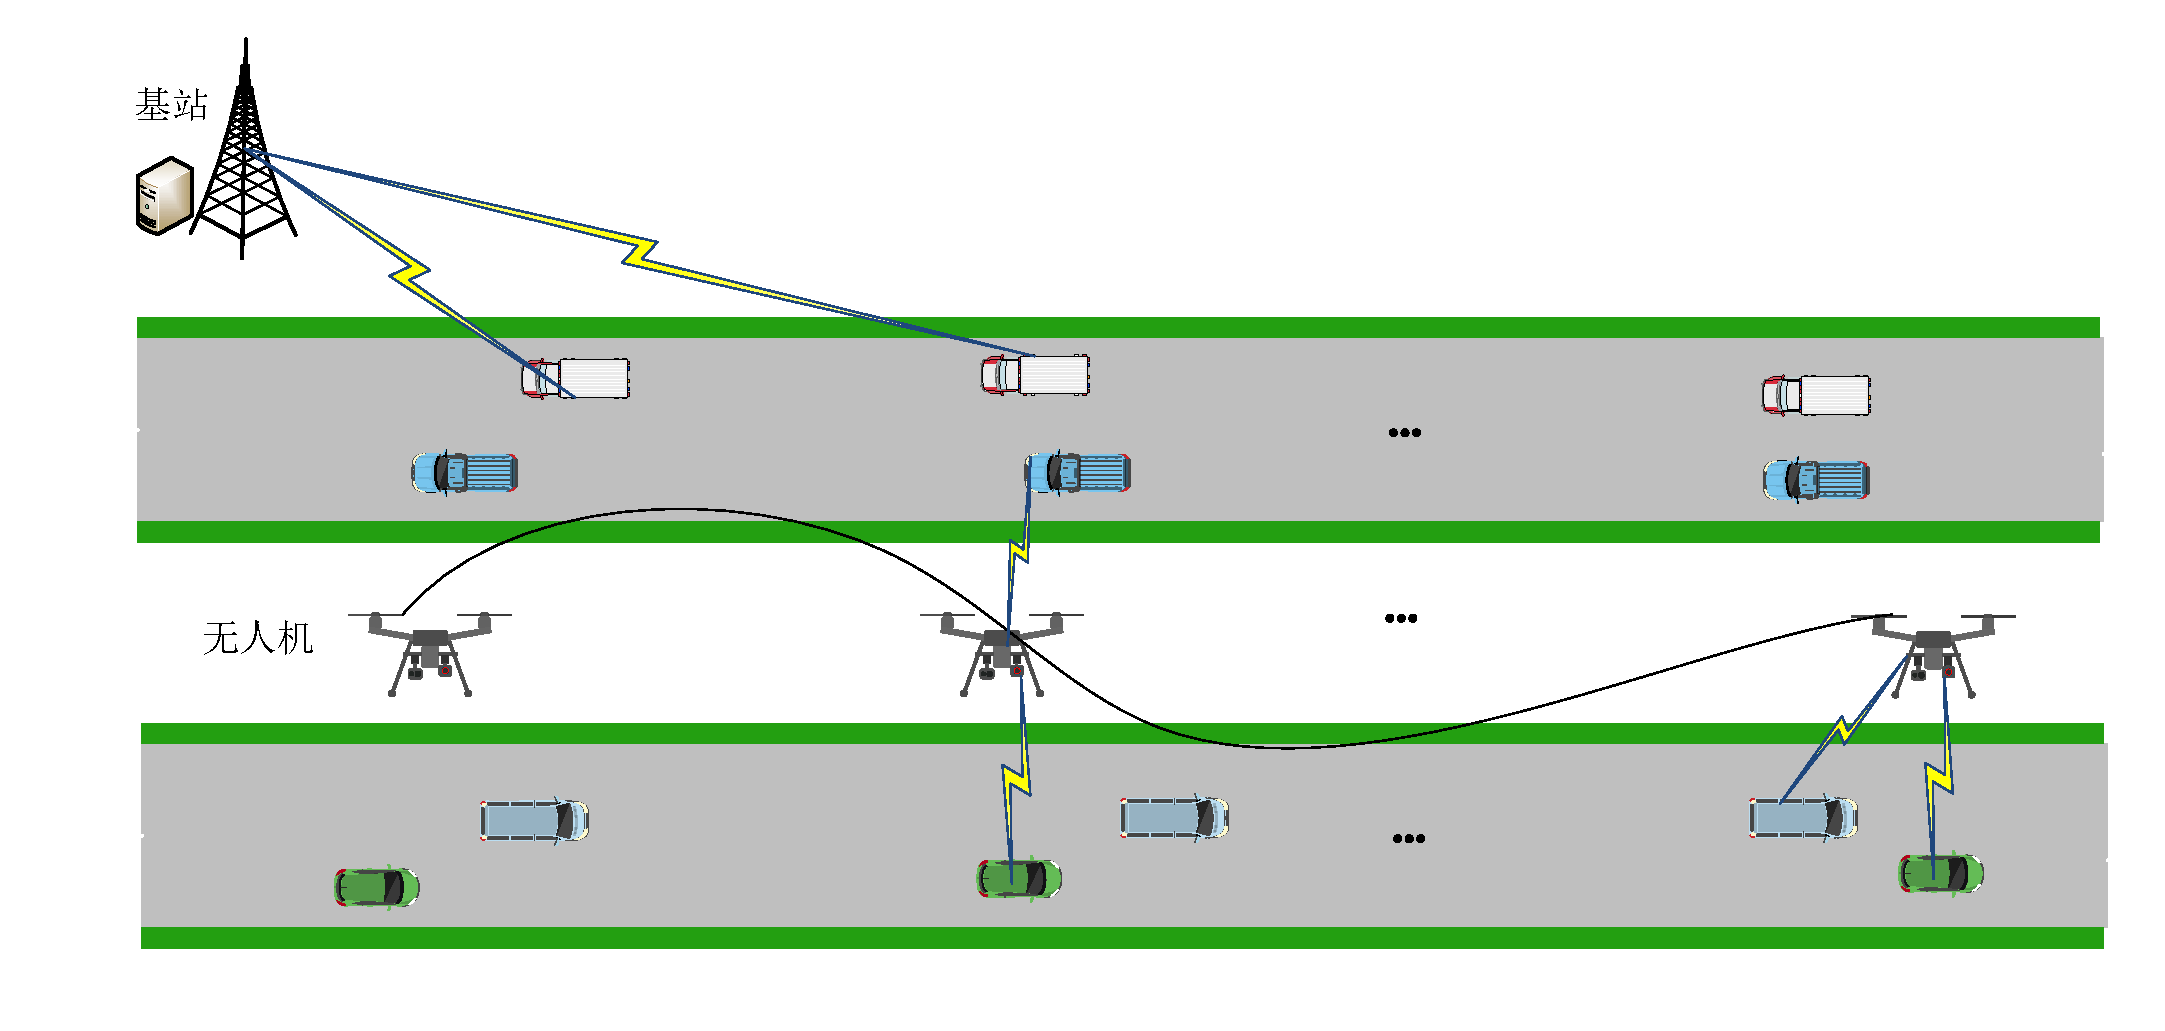
\includegraphics[width=12cm,height=8cm]{figures//chap4//第四章系统模型图.pdf}
\caption{无人机的系统模型}
\label{systemuav2}
\end{figure}

\subsection{车辆与地面基站通信与能耗模型}\label{section4-2-1}
由于车辆移动的快速性,对于车辆与路边单元的V2I通信,构建类似于前一章的一阶马尔可夫过程,在第$t$ 时刻的信道状态信息由前一时刻的状态预测得出,
即
\begin{equation} \label{E4-1}
%{\widetilde{g}}_{i,j}^k=L_{i,j}^2{\widetilde{h}}_{i,j}^2\xi_{i,j}^2
%h=\xi\tilde{h}+\sqrt{1-{{\xi }^{2}}}\zeta\    {\widetilde{g}}_{i,j}^k=L_{i,j}^2{\widetilde{h}}_{i,j}^2\xi_{i,j}^2
%{\widetilde{h}}_{m,R}=L_{m,R}^2{\widetilde{h}}_{m,R}^2\xi_{m,R}^2
h_{m}={\widetilde{h}}_{m}^2+{\hat{h}_{m}}^2,
\end{equation}
这里的${\widetilde{h}}_{m}$ 是一个观测值,${\hat{h}}_{m}$ 是一个服从参数为$a=\frac{1}{{L_{i,j}^t}({1-{\zeta_{i,j}^t}^2})}$ 的指数分布,其中$\zeta$ 表示信道增益,其复高斯分布为 $\zeta\sim CN\left(0,\delta^2\right)$,
$ {L_{i,j}^t}^2 $表示第 $t $ 个时隙的大规模衰减效应,包括阴影衰减路径损耗。
在第$t$ 个时隙,地面基站收到的第$m$辆车的信噪比SNR可以表示为:
\begin{equation} \label{E4-2}
\gamma_{m,R}\left[t\right]=\frac{p_m\left[t\right]h_{m,R}\left[t\right]}{\sigma^2}
\end{equation}
根据香农容量定理,车辆向地面基站的传输速率可以表示为:
\begin{equation} \label{E4-3}
R_{m,R}\left[t\right]=\log_2{\left(1+\gamma_{m,R}\left[t\right]\right)}
\end{equation}
车辆向地面基站传输的数据量可以表示为,
\begin{equation} \label{E4-4}
{{L}_{m,R}}={{B}_{0}}\underset{m=1}{\overset{M}{\mathop{\sum }}}\,\underset{t=1}{\overset{T}{\mathop{\sum }}}\,{{x}_{m}}\left[ t \right]R_{m,R}\left[t\right]
\end{equation}
其中$B_0$表示带宽,${{x}_{m}}\left[ t \right]=1$ 表示车辆当前时刻选择向地面基站传输数据。%${{x}_{m}}\left[ t \right]=0$ 反之。

车辆向地面基站路边单元通信时的传输能耗计算如下:
\begin{equation} \label{E4-6}
{{E}_{m,R}}=\underset{m=1}{\overset{M}{\mathop{\sum }}}\,\underset{t=1}{\overset{T}{\mathop{\sum }}}\,{{x}_{m}}\left[ t \right]{{p}_{m}}\left[ t \right]\
\end{equation}
\subsection{车辆与无人机通信与能耗模型}\label{section4-2-2}
对于车辆与无人机之间的通信中间没有障碍物遮挡,属于视距链路,构建了空中射频链路模型,
在第$t$ 个时隙,第$m$个车辆到无人机的信道增益为
\begin{equation} \label{E4-7}
h_{m,U}\left[t\right]=\frac{\varsigma_0}{{d_{m,U}\left[t\right]}^2}
\end{equation}
这里的$\varsigma_0$ 为单位距离1米下的功率增益,
%无人机与第$m$ 辆车之间的实时动态距离通过以下公式计算:
通过以上信息,无人机到车辆的传输速率为
\begin{equation} \label{E4-8}
R_{m,U}\left[t\right]=\log_2{\left(1+\gamma_{m,U}\left[t\right]\right)}
\end{equation} 其中
\begin{equation} \label{E4-9}
\gamma_{m,U}\left[t\right]=\frac{p_m\left[t\right]h_{m,U}\left[t\right]}{\sigma^2}
\end{equation} 表示车辆到无人机通信的信噪比,车辆向无人机空中基站传输的数据量可以表示为
\begin{equation} \label{E4-10}
%{{L}_{m,U}}={{B}_{0}}\underset{m=1}{\overset{M}{\mathop{\sum }}}\,\underset{t=1}{\overset{T}{\mathop{\sum }}}\,{{x}_{m}}\left[ t \right]{{\log }_{2}}\left( 1+{\gamma_{m,U}}\left[ t \right] \right)\
{{L}_{m,U}}={{B}_{0}}\underset{m=1}{\overset{M}{\mathop{\sum }}}\,\underset{t=1}{\overset{T}{\mathop{\sum }}}\,{{x}_{m}}R_{m,U}\left[t\right]
\end{equation}
其中$B_0$表示带宽,车辆向空中基站无人机通信时的传输能耗计算如下:
\begin{equation} \label{E4-11}
{{E}_{m,U}}=\underset{m=1}{\overset{M}{\mathop{\sum }}}\,\underset{t=1}{\overset{T}{\mathop{\sum }}}\,{{y}_{m}}\left[ t \right]{{p}_{m}}\left[ t \right]\
\end{equation}
由于无人机与路边单元之间具有良好的视距链路,因此可以认为车辆发送给无人机的数据
可以高效的传输到地面基站并由路边单元附属的边缘服务器进行数据处理。
\subsection{车辆计算任务卸载模型}\label{section4-2-44}
附属于路边单元的边缘服务器可以为收到的车辆数据进行数据计算处理
,因此计算卸载过程需要计算
资源,执行协作计算模型分裂的子任务。第$m$个车辆
的整个计算任务记为$A_m$,在某个时隙当其将任务分给路边单元时记为:
$A_{R,m}={{z}_{m}}A_m$
定义$f_R$是路边单元的边缘服务器的CPU的加速频率,则计算时间可以表示为:
\begin{equation} \label{E4-5}
t_{m}^{mec}=\frac{A_{R,m}}{f_R}% \quad m \in \mathcal{M}.
\end{equation}
车辆完成任务上传与计算的时间为路边单元向边缘服务器发送数据时的固定时间与计算时间之和,为保证任务顺利传输并计算,该时间应小于车辆
在单元覆盖范围内的行驶时间。

第 $m$ 个需要上传其子任务后边缘服务器的计算能耗为:
\begin{equation} \label{E4-55}
E_{m}^{mec}=\aleph A_{R,m}{f_R}^2% \quad m \in \mathcal{M}.
\end{equation}
其中,$\aleph > 0 $是 CPU 的有效开关电容,取决于芯片结构。
%同时我们使用瞬时的传输速率代替平均上传速率,由此可以得到车辆任务的上传时间为:、
%这里,我们将网络效用H(Am,i) 定义为与访问子任务相关的卸载任务的计算满意度  车辆完成任务上传与计算的时间为路边单元向边缘服务器发送数据时的固定时间与计算时间之和
\subsection{能效最大化问题的定义}\label{section4-2-3}
在本节中,为无人机辅助的双向车道车辆制定了能效最大化问题。目的是通过联合优化双向车道
上的车辆的发射功率以及无人机的轨迹来使得系统的总能效最大化.
首先,该网络通信系统的能效定义为
\begin{equation} \label{E4-12}
EE(\mathbf{P}, \mathbf{Q}, \mathbf{X})=
{\frac{{{L}_{m}}\left( \mathbf{P}, \mathbf{Q}, \mathbf{X} \right)}
{{{E}_{m}}\left( \mathbf{P}, \mathbf{X} \right)}}
%EE(P,Q)=\sum\limits_{m=1}^{M}{\sum\limits_{n=1}^{N}{\frac{{{L}_{m,R}}\left[ n \right]+{{L}_{m,U}}\left[ n \right]}{{{E}_{m}}\left[ n \right]}}}
\end{equation}
式中的${{L}_{m}={L}_{m,R}+{L}_{m,U}}$ 是车辆向地面基站与空中基站发送的总的数据量,${E}_{m}$ 包括车辆与地面基站空中基站的能量消耗与边缘服务器的计算能耗。
由于无人机飞行过程中会有能量的消耗,因此应更加关注车辆与无人机通信时的能耗问题,并考虑空中基站通信与地面基站通信的能量权衡,
因此系统的总功耗表示为${{E}_{m}=E_{m}^{mec}+(1-\theta){L}_{m,R}+\theta{L}_{m,U}}$,其中$0\le \theta \le 1$是车辆与无人机通信时的能量成本的权重系数。
当$\theta$ 较大时意味着更加关注无人机的能耗成本。
最终的系统能效最大化问题如下表述:
\begin{align}
& \qquad\qquad\textbf{P}:\qquad \max_{ \mathbf{P}, \mathbf{Q}, \mathbf{X} }  EE(\mathbf{P}, \mathbf{Q}, \mathbf{X})                \label{E4-13}\\
\text { s.t. }
& \Pr\left\{x_m\left[t\right]\gamma_{m,R}\left[t\right]+y_m\left[t\right]\gamma_{m,U}\left[t\right]\geq \gamma_{th}\right\}\geq1-\varepsilon_3, \forall m,t   \tag{\ref{E4-13}{-1}}      \label{E4-13-1}\\  %信噪比中断概率约束
& 0\le p_m\left[t\right]\le p_{max}, \forall m,t                           \tag{\ref{E4-13}{-2}}      \label{E4-13-2}\\  %功率阈值
& x_m\left[t\right] + y_m\left[t\right]=1, \forall m,t                     \tag{\ref{E4-13}{-3}}      \label{E4-13-3}\\  %时隙分配加起来是一
& \frac{D_R}{\nu_m} \geq t_{m}^{mec}+t_{wired} , \forall m,t                           \tag{\ref{E4-13}{-4}}      \label{E4-13-4}\\  %这个是时隙的约束
& q_U^{n\mathrm{\ }+1}-q_U^{n\mathrm{\ }}\le tV_{max}, \forall m,t         \tag{\ref{E4-13}{-5}}      \label{E4-13-5}    %无人机飞行轨迹
\end{align}

上式子中的\eqref{E4-13-1} 表示了保证车辆通信的中断概率约束来保证服务质量,式子\eqref{E4-13-2} 给出了
车辆最大最小发射功率的约束,式\eqref{E4-13-3} 则代表了每个车辆每个时刻的任务只能向无人机或者地面基站
进行卸载,$\gamma_{th}$ 是信噪比的阈值为一个固定值,%表示了需要调度车辆在其驶出路边单元覆盖范围之前服务器要完成完成数据的计算,
%可以通过约束 \eqref{E4-13-4} 进行时隙资源的分配,
式 \eqref{E4-13-4} 表示了需要调度车辆在其驶出路边单元覆盖范围之前服务器要完成完成
数据的计算,可以通过此约束进行时隙资源的分配,
其中$t_{wired}$ 是路边单元向边缘服务器发送数据时的
固定时间。无人机的飞行轨迹受到 \eqref{E4-13-5} 的约束,即无人机每秒的实际飞行距离要小于等于无人机最大可飞行距离。

\section{能效最大化问题求解}\label{section4-3}
在本节中,上一章节的能效最大化问题会分解为两个子问题进行求解。对于难以求解的分式规划,可以使用丁克尔巴赫方法
将其转化为易于求解的减式规划进行求解。首先固定车辆的发射功率后求解无人机的飞行轨迹,然后固定无人机的飞行轨迹再求解
车辆的发射功率,如此进行交替迭代优化,直至算法收敛。注意到前一节中问题\eqref{E4-13} 是一个非凸的问题,本节提出了
一种联合功率分配与无人机轨迹规划的方案来有效地处理这个问题,将问题\eqref{E4-13} 解耦成三个子问题 \cite{JointTrajectory9627548}。
\subsection{概率约束的近似与车辆发射功率优化问题}\label{section4-3-1}
在前一节的式\eqref{E4-13-1} 中可以发现车辆的功率功率在概率约束中存在较为复杂的耦合关系,是难以直接求解的,
针对这种情况,将采用积分变换的方式将复杂的概率约束问题转化为较为简单的形式。

%\begin{theorem}[定理:]
%\end{theorem}
对于\eqref{E4-13-1},车辆用户的中断概率约束
\begin{align}
\Pr\left\{x_m\left[t\right]\gamma_{m,R}\left[t\right]+y_m\left[t\right]\gamma_{m,U}\left[t\right] \geq \gamma_{th}\right\}\geq1-\varepsilon_3    \notag
\end{align}
等价于:
\begin{equation} \label{E4-14}
\begin{gathered}
p_m\left[t\right]x_m\left[t\right]\ln \left(1-a \varepsilon_3\right)+(\gamma_{th}-y_m\left[t\right]\gamma_{m,U})\left[t\right] a \sigma^2
\leq a p_m\left[t\right]x_m\left[t\right]\hat{h}_{m}\left[t\right]
\end{gathered}
\end{equation}
%\textcolor[RGB]{202,12,22}{巴拉巴拉}
%\begin{proof}
%\end{proof}
\textbf{证明}: 由 \eqref{E4-1} 和\eqref{E4-13-1} 可得
\begin{align} \label{E4-15}
\qquad & \frac{x_m[t]p_m[t]h_{m,R}[t]}{\sigma^2} \geq \gamma_{th} - y_m[t]\gamma_{m,U}[t] \\
\Leftrightarrow \quad
& p_m[t]{\widetilde{h}}_{m}[t] \geq \frac{(\gamma_{th} - y_m[t]\gamma_{m,U}[t])\sigma^2}{x_m[t]} - p_m[t]{\hat{h}}_{m}[t] \notag
\end{align}
%$\frac{{(SNR_{th}-y_m\left[t\right]\gamma_{m,U})\sigma^2}}{x_m\left[t\right]}$
因此车辆用户的中断概率约束做出重新表述如下:
\begin{align} \label{E4-16}
\Pr\left\{ x_m[t]\gamma_{m,R}[t] + y_m[t]\gamma_{m,U}[t] \geq \gamma_{th} \right\} &\geq 1 - \varepsilon_3 \\
\Leftrightarrow \quad
\Pr\left\{ {\widetilde{h}}_{m}[t] \geq \frac{(\gamma_{th} - y_m[t]\gamma_{m,U}[t])\sigma^2}{p_m[t]x_m[t]} - {\hat{h}}_{m}[t] \right\} &\geq 1 - \varepsilon_3 \notag
\end{align}
由于随机变量$\widetilde{h}$ 的概率密度函数为$f_x={{e}^{-ax}}$,通过积分变换可得:
\begin{align} \label{E4-17}
\int_{0}^{\frac{(\gamma_{th}-y_m[t]\gamma_{m,U})\sigma^2}{p_m[t]x_m[t]} - \hat{h}_{m}[t]}{e^{-ax}dx} &\leq \varepsilon_3  \\
\Leftrightarrow \quad
p_m[t]x_m[t]\ln(1-a\varepsilon_3) + (\gamma_{th}-y_m[t]\gamma_{m,U}[t])a\sigma^2 &\leq a p_m[t]x_m[t]\hat{h}_{m}[t] \notag
\end{align}
%GVRR.* P_m.*X' >= SNRth*Delta+ GVUU.*P_m.*Y'+log(1-e1)*P_m.*X'

为了表达方便,定义  %另起一段
$\gamma_{m,U}\left[t\right]=p_m\left[t\right]\eta_{m,U}\left[t\right]$,其中$\eta_{m,U}\left[t\right]=h_{m,U}\left[t\right]/{\sigma^2}$,进一步的可得:
\begin{equation} \label{E4-1833}
{{\kappa }_{m}}\left[ t \right]={{x}_{m}}\left[ t \right]\ln \left( 1-a{{\varepsilon }_{3}} \right)-{{y}_{m}}\left[ t \right]{{\eta }_{m,U}}\left[ t \right]a{{\sigma }^{2}}-a{{x}_{m}}\left[ t \right]{{\hat{h}}_{m}}\left[ t \right]
\end{equation}
 并将式子 \eqref{E4-17} 改写为:%\par
%\textcolor[RGB]{202,12,22}{这里不太对}
\begin{equation} \label{E4-18}
{{p}_{m}}\left[ t \right]{{\kappa }_{m}}\left[ t \right]+a{{\sigma }^{2}}{{\gamma }_{th}}\le 0
%p_m\left[t\right]x_m\left[t\right]\ln \left(1-a \varepsilon_3\right)+(\gamma_{th}-y_m\left[t\right]p_m\left[t\right]\eta_{m,U}\left[t\right]) a \sigma^2
%\leq a p_m\left[t\right]x_m\left[t\right]\hat{h}_{m}\left[t\right]
\end{equation}
在求解车辆发射功率的过程中,需要每个时隙都要进行功
率分配与无人机轨迹规划并进行多次迭代,
关于车辆发射功率$p_m\left[t\right]$ 的子问题如下描述:
\begin{align}  \label{E4-19}
\max _{ \mathbf{P}} &   ={\frac{{{L}_{m}}\left( \mathbf{P} \right)}
{(1-\theta){E}_{m,R}\left( \mathbf{P} \right)+\theta{E}_{m,R}\left( \mathbf{P} \right)}}        \\
&\text { s.t. }
%& \eqref{E4-3end1},\eqref{E4-3end4}        \tag{\ref{E4-4end}{-1}}      \label{E4-4end1}
 \eqref{E4-18},\eqref{E4-13-2}                                                  \tag{\ref{E4-19}{-1}}      \label{E4-19-1}
\end{align}
注意到问题\eqref{E4-19} 是一个分式规划问题,
%\textcolor[RGB]{202,12,22}{该该算法的主要思想是将原始非线性规划问题转化为一个系列的线性规划问题,然后使用线性规划的解法来逼近非线性规划问题的解。具体步骤可能因问题而异,但总体上,该方法尝试通过不断调整问题中的某些参数来逐步优化目标函数。}
为了将其转化为减式规划问题,拟采用丁克尔巴赫方法求解,通过引入一个辅助变量,将原始的非线性规划问题转化为线性规划问题。然后,通过逐步迭代更新辅助变量的值,直到满足特定的收敛条件,从而找到目标函数的最优解。
问题\eqref{E4-19} 转化为:
\begin{align} \notag
F(\chi)&=  \max _{ \mathbf{P}} \sum_{t=1}^T \sum_{m=1}^M {B}_{0}x_{m}^{\left\{ l \right\}}\left[ t \right] %x_m\left[t\right]
\log_2{\left(1+p_m\left[t\right]\eta_{m,R}^{\left\{ l \right\}}\left[t\right]\right)}                         \\       \label{E4-20}
& -\chi \sum_{t=1}^T \sum_{m=1}^M{(1-\theta)x_{m}^{\left\{ l \right\}}\left[ t \right]p_m\left[t\right]
+\theta y_{m}^{\left\{ l \right\}}\left[ t \right]p_m\left[t\right]}                           \\ \notag
& + \sum_{t=1}^T \sum_{m=1}^M {B}_{0}y_{m}^{\left\{ l \right\}}\left[ t \right]
\log_2{\left(1+p_m\left[t\right]\eta_{m,U}^{\left\{ l \right\}}\left[t\right]\right)}                                          \\ \notag
&\text { s.t. }
 \eqref{E4-18},\eqref{E4-13-2}                                                           \tag{\ref{E4-20}{-1}}       \label{E4-20-1}
%& \eqref{E4-3end1},\eqref{E4-3end4}                                       \tag{\ref{E4-5end}{-1}}                      \label{E4-5end1}
\end{align}
上式中的$\eta_{m,R}^{\left\{ l \right\}}\left[t\right]=h_{m,R}\left[t\right]/{\sigma^2}$,
$\eta_{m,U}^{\left\{ l \right\}}\left[t\right]=h_{m,U}\left[t\right]/{\sigma^2}$
在每$l$ 次迭代时视为常数,对于凸问题\eqref{E4-20},
可以构建拉格朗日函数并运用拉格朗日对偶法进行求解:
\begin{align} \label{E4-21}
&\!\!\!\!\!\!L\left(\mathbf{p},\lambda\right)=B_{0}\sum_{t=1}^{T} \sum_{m=1}^{M}  \!\! x_{m}^{\{ l \}}[t] \log_{2}\left(1 + p_{m}[t]\eta_{m,R}^{\{ l \}}[t]\right) \! +\!  y_{m}^{\{ l \}}[t] \log_{2}\left(1 + p_{m}[t]\eta_{m,U}^{\{ l \}}[t]\right)  \\
&\!\!\!\!\!\!-\chi \sum_{t=1}^T \sum_{m=1}^M{(1-\theta)x_{m}^{\left\{ l \right\}}\left[ t \right]p_m\left[t\right]
+\theta y_{m}^{\left\{ l \right\}}\left[ t \right]p_m\left[t\right]} % \\ 如果换了下面一行的话要取消这个注释
-\sum\limits_{t=1}^{T}{\sum\limits_{m=1}^{M}{{{\lambda }_{m,t}}}}\left( {{p}_{m}}\left[ t \right]{{\kappa }_{m}}\left[ t \right]+a{{\sigma }^{2}}{{\gamma }_{th}} \right) \notag
\end{align}

其中的拉格朗日乘子$\lambda_{m,t}\geq 0$,则\eqref{E4-21} 的拉格朗日对偶函数表示为:
\begin{equation} \label{E4-22}
D(\mathbf{\lambda})=\max _{\substack{0 \leq P_m[t] \leq P_{\max }}} L\left(\mathbf{p_m},\mathbf{\lambda}\right)
\end{equation}
其中\eqref{E4-22} 的对偶问题为:
\begin{equation} \label{E4-23}
\min_{\substack{\lambda_{m,t}\geq 0}} D\left(\mathbf{p_m},\mathbf{\lambda}\right)
\end{equation}
问题\eqref{E4-23} 是一个凸问题且满足Karush-Kuhn-Tucker(KKT)条件,
在使用KKT条件的类似求解过程中可令其一阶导数为等于零:
\begin{align}\label{E4-24}
\frac{{{B}_{0}}x_{m}^{\left\{ l \right\}}\left[ t \right]\eta _{m,R}^{\left\{ l \right\}}\left[ t \right]}{\ln 2\left( 1+{{p}_{m}}\left[ t \right]\eta _{m,R}^{\left\{ l \right\}}\left[ t \right] \right)}+\frac{{{B}_{0}}y_{m}^{\left\{ l \right\}}\left[ t \right]\eta _{m,U}^{\left\{ l \right\}}\left[ t \right]}{\ln 2\left( 1+{{p}_{m}}\left[ t \right]\eta _{m,U}^{\left\{ l \right\}}\left[ t \right] \right)}+\chi \left( \theta -x_{m}^{\left\{ l \right\}}\left[ t \right] \right) \\   \notag
%-\sum\limits_{t=1}^{T}{{{\lambda }_{m,t}}}\left( {{p}_{m}}\left[ t \right]{{\kappa }_{m}}\left[ t \right]+a{{\sigma }^{2}}{{\gamma }_{th}} \right)=0
-\sum\limits_{t=1}^{T}{{{\lambda }_{m,t}}}\left( -{{y}_{m}}[t]{{\eta }_{m,U}}[t]a{{\sigma }^{2}}+{{x}_{m}}[t]{{{\hat{h}}}_{m}}[t]-\frac{{{x}_{m}}[t]a{{\varepsilon }_{3}}}{1-a{{\varepsilon }_{3}}} \right)=0,
\end{align}
由上式可得
\begin{align}\label{E4-25}
\!\!\!\!{{p}_{m}}\left[ t \right]=\frac{x_{m}^{\left\{ l \right\}}\left[ t \right]}{\eta _{m,R}^{\left\{ l \right\}}\left[ t \right]}+\frac{y_{m}^{\left\{ l \right\}}\left[ t \right]}{\eta _{m,U}^{\left\{ l \right\}}\left[ t \right]}-\frac{{{B}_{0}}}{\ln 2{{\lambda }_{m,t}}\left[ y_{m}^{\left\{ l \right\}}\left[ t \right]\eta _{m,U}^{\left\{ l \right\}}\left[ t \right]a{{\sigma }^{2}}+x_{m}^{\left\{ l \right\}}\left( {{{\hat{h}}}_{m}}[t]-\frac{a{{\varepsilon }_{3}}}{1-a{{\varepsilon }_{3}}} \right) \right]}
\end{align}
为了简化表达,令${{c}_{m}}\left[ t \right]=y_{m}^{\left\{ l \right\}}\left[ t \right]\eta _{m,U}^{\left\{ l \right\}}\left[ t \right]a{{\sigma }^{2}}+x_{m}^{\left\{ l \right\}}\left( {{{\hat{h}}}_{m}}[t]-\frac{a{{\varepsilon }_{3}}}{1-a{{\varepsilon }_{3}}} \right)$,

根据 \eqref{E4-24},功率分配通过以下方式迭代更新,
\begin{align} \label{E4-26}
{{p}_{m}}{{\left[ t \right]}^{*}}=\left[ \frac{x_{m}^{\left\{ l \right\}}\left[ t \right]}{\eta _{m,R}^{\left\{ l \right\}}\left[ t \right]}+\frac{y_{m}^{\left\{ l \right\}}\left[ t \right]}{\eta _{m,U}^{\left\{ l \right\}}\left[ t \right]}-\frac{{{B}_{0}}}{\ln 2{{\lambda }_{m,t}}{{c}_{m}}\left[ t \right]} \right]_{0}^{{{p}_{max}}\ }
\end{align}
可以用次梯度法更新拉格朗日乘数 $\lambda_m$ ,具体方法如下:
\begin{equation}\label{E4-27}
\lambda _{m}^{\left( i+1 \right)}={{\left[ \lambda _{m}^{\left( t \right)}+\Delta _{m}^{\left( t \right)}{{G}_{{{\lambda}_{m}}}} \right]}^{+}}
%\lambda_m^{\left(i+1\right)}=\left[\lambda_m^{\left(t\right)}+K_\lambda^{\left(i\right)}\left(\sum_{j\neq i}^{M}{\chi_{i,j}e^{{\widetilde{p}}_j}}+\mathrm{\Pi}_i\right)\right]^+,
\end{equation}

其中 ${{G}_{{{\lambda}_{m}}}}$ 代表拉格朗日乘法器的步长,且${{G}_{{{\lambda}_{m}}}}\geq0$ 。
变量 $i$ 是迭代指数,变量 $x$ 的正部分定义为 $\left[x\right]^+=\max{\left[0,x\right]} $ 。
%$\lambda _{m}^{\left( i+1 \right)}={{\left[ \lambda _{m}^{\left( t \right)}+\Delta _{m}^{\left( t \right)}{{G}_{{{\lambda}_{m}}}} \right]}^{+}}$
拉格朗日乘子由次梯度法更新如下,
\begin{equation}\label{E4-28}
{{G}_{{{\lambda }_{m}}}}={{p}_{m}}\left[ t \right]{{\kappa }_{m}}\left[ t \right]+a{{\sigma }^{2}}{{\gamma }_{th}}
\end{equation}
%\textcolor[RGB]{202,12,22}{再加上橙子梯度}
\subsection{计算时间约束转化与时隙资源分配问题}\label{section4-3-3}
由式 \eqref{E4-13-4} 与$A_{R,m}={{z}_{m}}A_m$,时隙的分配受到服务器计算时间的制约,可得:
\begin{equation} \label{E4-35}
{{z}_{m}}=\underset{t=1}{\overset{T}{\mathop{\sum }}}{{x}_{m}}\left[ t \right]   ,\qquad\forall \!\!\!\!\!\! \quad m \in \mathcal{M}
\end{equation}
即车辆向地面基站通信的所有的时隙加起来要小于
车辆在基站的覆盖范围内。当功率 和轨迹 {}给定时,关于分配时隙的子问题如下:
\begin{align} \label{E4-36}
\max _{ \mathbf{X},\mathbf{Y}}  &  ={\frac{{{L}_{m,R}\left( \mathbf{X} \right)+{{L}_{m,U}}\left( \mathbf{Y} \right)}}
{(1-\theta){{E}_{\text{t}}}^{R,\left\{ l \right\}}\left( \mathbf{X} \right)+\theta{{E}_{\text{t}}}^{U,\left\{ l \right\}}\left( \mathbf{Y} \right)}}     \\
\text { s.t. }
& \eqref{E4-13-3},\eqref{E4-13-4}                                                        \tag{\ref{E4-36}{-1}}           \label{E4-36-1}
\end{align}
这是一个分式规划的问题,可以使用与问题 \eqref{E4-19} 类似的丁克尔巴赫方法将原问题转化为
易于求解的减式规划,即式子 \eqref{E4-36} 等价于一个可以使用凸优化工具箱(CVX)迭代求解的线性规划问题。
\subsection{无人机飞行轨迹规划问题}\label{section4-3-2}
%\textcolor[RGB]{202,12,22}{ }
求得车辆功率的分配后,对于无人机轨迹的优化问题,
当每次迭代的车辆发射功率$\left\{ {{P_m}^{\left\{ l \right\}}} \right\}$ 和时隙分配
%无人机的轨迹$\left\{ {{Q}^{\left\{ l \right\}}} \right\}$
给定后,关于无人机的轨迹的优化描述如下:
\begin{align} \label{E4-29}
\max _{ \mathbf{Q}} &   ={\frac{{{L}_{m,R}+{{L}_{m,U}}\left( \mathbf{Q} \right)}}
{(1-\theta){{E}_{\text{t}}}^{R,\left\{ l \right\}}+\theta{{E}_{\text{t}}}^{U,\left\{ l \right\}}}}        \\
\text { s.t. }
& \eqref{E4-13-5}                                                       \tag{\ref{E4-29}{-1}}           \label{E4-29-1}
\end{align}
其中,
\begin{equation} \label{E4-30}
{{L}_{m,U}}\left( \mathbf{Q} \right)={{\log }_{2}}\left( 1+\frac{\varphi _{m,U}^{\{l\}}\left[ t \right]}{\left\| {{q}_{M}}\left[ t \right]-{{q}_{U}}\left[ t \right] \right\|+{{H}^{2}}} \right)\
\end{equation}
这里的${\varphi _{m,U}^{\{l\}}\left[ t \right]}=\frac{p_{_{m}}^{\{l\}}\left[ t \right]\varsigma_0}{\sigma^2}$,
注意到问题\eqref{E4-29} 目标函数的分子部分是非凹问题,拟采用连续凸逼近方法对目标函数进行近似。在
${{q}^{\left\{ l \right\}}}\left[t\right]$
的局部点处,对式\eqref{E4-29} 的分子部分的对数形式进行一阶泰勒展开,过程如下:
\begin{align} \label{E4-31}
&{{\log }_{2}}\left( 1+\frac{\varphi _{m,U}^{\{l\}}\left[ t \right]}{\left\| {{q}_{M}}\left[ t \right]-{{q}_{U}}\left[ t \right] \right\|+{{H}^{2}}} \right)\ \\    \notag
&\geq\left(\omega _{_{m}}^{\{l\}}\left[ t \right] {{\left\| {{q}_{M}}\left[ t \right]-{{q}_{U}}\left[ t \right] \right\|}^{2}}-{{\left\| {{q}_{M}}\left[ t \right]-q_{U}^{\{l\}}\left[ t \right] \right\|}^{2}}+\rho _{m}^{\{l\}}\left[ t \right] \right) \\  \notag
&\triangleq R_{m,U}^{\{l\}}(\mathbf{q}[t])  \notag
\end{align}
其中,
\begin{align} \label{E4-32}
\omega _{_{m}}^{\{l\}}\left[ t \right]=\frac{-\varphi _{m,U}^{\{l\}}\left[ t \right]}{\ln 2\left( {{\left\| {{q}_{M}}\left[ t \right]-q_{U}^{\{l\}}\left[ t \right] \right\|}^{2}}+{{H}^{2}} \right)}\cdot \frac{1}{{{\left\| {{q}_{M}}\left[ t \right]-q_{U}^{\{l\}}\left[ t \right] \right\|}^{2}}+{{H}^{2}}+\varphi _{m,U}^{\{l\}}\left[ t \right]}
\end{align}
并且,
\begin{equation} \label{E4-33}
\rho_{_{m}}^{\{l\}}\left[ t \right]={{\log }_{2}}\left( 1+\frac{\varphi _{m,U}^{\{l\}}\left[ t \right]}{\left\| {{q}_{M}}\left[ t \right]-q_{U}^{\{l\}}\left[ t \right] \right\|+{{H}^{2}}} \right)\
\end{equation}
问题 \eqref{E4-29} 进一步转化为:
\begin{align} \label{E4-34}
\max _{ \mathbf{Q}}  &  ={\frac{{{L}_{m,R}+\sum\limits_{t=1}^{T}{\sum\limits_{m=1}^{M}{{{B}_{0}}}}y_{m}^{\left\{ l \right\}}\left[ t \right]R_{m,U}^{\{l\}}(\mathbf{q}[t])}}
{(1-\theta){{E}_{\text{t}}}^{R,\left\{ l \right\}}+\theta{{E}_{\text{t}}}^{U,\left\{ l \right\}}}}       \\
\text { s.t. }
& \eqref{E4-13-5}                                                       \tag{\ref{E4-34}{-1}}           \label{E4-34-1}
\end{align}
类似于问题 \eqref{E4-36},问题 \eqref{E4-29} 的非凸问题部分转化成了凸问题,并且是容易求解的形式,可以使用CVX 工具箱进行迭代求解。%再加一行行不行再加一行行不行再加一行行不行再加一行行不行再加一行行不行再加一行行不行再加一行行不行行不行再加一行

%\textcolor[RGB]{202,12,22}{与(3-17)类似,(3-31)中的分数形式的目标函数可以通过丁克尔巴赫方法转换为减法形式,因此可以通过使用凸优化工具包(例如CVX[51]) 迭代解决。}
\begin{comment}  %这个也可以使用,就是字体有点粗
\begin{table}[htbp!]
 \centering\small
 \renewcommand\arraystretch{1.5}   %latex 三线表中各行间隔
 %\Tablecaption{系统仿真参数}\label{biao42}
\begin{tabular*}{\hsize}{@{\extracolsep{\fill}}l l l l}
 \toprule
 算法4-3 基于固定节点功率分配的无人机轨迹优化方案           \\
 \midrule
    Step1:开始。                                      \\
    Step2:输入功率矩阵$P$ 和车辆分簇信息$C$            \\
   Step3:地面基站高度面基站高度面基站高度面基站高度  \\
    Step4:计算无人机轨迹                              \\
    Step5:地面基站高度面基站高度面基站高度面基站高度  \\
    Step6:执行$l=l+1$                         \\
   Step7:重复执行Step3 至Step5,直到满足收敛条件      \\
    Step8:结束。                         \\
 \bottomrule
 \end{tabular*}
\end{table}
\end{comment}
\section{算法与仿真验证}\label{section4-5}
\subsection{总体算法设计}\label{section4-5-1}
原始的问题\eqref{E4-13} 被分为三个子问题,分别为车辆发射功率优化问题、时隙资源分配问题以及无人机飞行轨迹规划问题,它们均已在上述小节中分别得到解决。然后使用交替迭代的方法交替求解,该算法如下所示,
\begin{center}
\begin{tabular*}{\hsize}{@{\extracolsep{\fill}}l l l l}
%\begin{tabular}{lcr}
    \toprule
    算法4-3 基于丁克尔巴赫方法的功率分配与无人机轨迹优化方案                  \\
    \midrule
    Step1:开始。                                                    \\
      Step2:初始化功率矩阵$P$,无人机轨迹$Q$ 和时隙资源的分配$X$       \\
           Step3:根据 \eqref{E4-26} 计算车辆的发射功率$ {{p}_{m}}{{\left[ t \right]}^{*}}$。                                      \\
          Step4:根据 \eqref{E4-34} 计算无人机轨迹$ {{Q}_{m}}{{\left[ t \right]}^{*}}$  。                                        \\
              Step5:根据 \eqref{E4-36} 确定时隙资源的分配$ {{X}_{m}}{{\left[ t \right]}^{*}}$。                                      \\
    Step6:执行更新$l=l+1$。                                         \\
    Step7:重复执行Step3 至Step6,直到满足收敛条件。                  \\
    Step8:结束。                                                   \\
    \bottomrule
\end{tabular*}
\end{center}


%\multicolumn{1}{c}{\centering 续表} \\ % 居中显示续表二字,并且不是粗体

\begin{comment}
\begin{table}[htbp!]
 \centering\small
% \Tablecaption{}\label{biao4-1}
\begin{tabular*}{\hsize}{@{\extracolsep{\fill}}c c c c}
 \toprule
 &&基于固定节点功率分配的无人机轨迹优化方案                   \\
 \midrule
 &&Step1:开始。                \\
 &&Step2:输入功率矩阵$P$和车辆分簇信息$C$               \\
 &&Step2:地面基站高度面基站高度面基站高度面基站高度                         \\
 \bottomrule
 \end{tabular*}
\end{table}

\begin{tabular}{lcr}
    \toprule
    Item  &amp; Quantity &amp; Price (\$) \\
    \midrule
    Apple &amp; 2        &amp; 1.50       \\
    Banana &amp; 3       &amp; 1.00       \\
    Cherry &amp; 5       &amp; 0.50       \\
    \bottomrule
\end{tabular}


\vspace*{0.2cm}% 设置了一点间距
\begin{tabular*}{\hsize}{@{\extracolsep{\fill}}l l l l}
%\begin{tabular}{lcr}
    \toprule
    算法4-3 基于固定节点功率分配的无人机轨迹优化方案                  \\
    \midrule
    Step1:开始。                                                    \\
    Step2:初始化功率矩阵$P$,无人机轨迹$Q$ 和时隙资源的分配$X$       \\
    Step3:根据 \eqref{E4-26} 计算车辆的发射功率$ {{p}_{m}}{{\left[ t \right]}^{*}}$。                                      \\
    Step4:根据 \eqref{E4-34} 计算无人机轨迹$ {{Q}_{m}}{{\left[ t \right]}^{*}}$  。                                        \\
    Step5:根据 \eqref{E4-36} 确定时隙资源的分配$ {{X}_{m}}{{\left[ t \right]}^{*}}$。                                      \\
    Step6:执行更新$l=l+1$。                                         \\
    Step7:重复执行Step3 至Step6,直到满足收敛条件。                  \\
    Step8:结束。                                                    \\
    \bottomrule
\end{tabular*}

删除的续表
\begin{center}
\begin{tabular*}{\hsize}{@{\extracolsep{\fill}}l l l l}
    \toprule
    \qquad\qquad\qquad\qquad\qquad\qquad\qquad\qquad\qquad 续表 \\ % 居中显示续表二字,并且不是粗体                  \\\multicolumn{1}{c}{\centering 续表}
    \midrule
  % Step3:根据 \eqref{E4-26} 计算车辆的发射功率$ {{p}_{m}}{{\left[ t \right]}^{*}}$。                                      \\
   %Step4:根据 \eqref{E4-34} 计算无人机轨迹$ {{Q}_{m}}{{\left[ t \right]}^{*}}$  。                                        \\
    Step5:根据 \eqref{E4-36} 确定时隙资源的分配$ {{X}_{m}}{{\left[ t \right]}^{*}}$。                                      \\
    Step6:执行更新$l=l+1$。                                         \\
    Step7:重复执行Step3 至Step6,直到满足收敛条件。                  \\
    Step8:结束。                                                    \\
    \bottomrule
\end{tabular*}
\end{center}
\end{comment}
\subsection{仿真分析}\label{section4-5-2}
在本小节中,为了检验算法的有效性并评估其性能,提供了数值仿真结果,主要评估了联合优化无人机轨迹和信道功率分配方案的性能,并介绍了
无人机固定位置悬浮方案与固定无人机轨迹的方式两种方案,并且将本章所提出的方案与之对比。
悬浮方案中无人机在固定位置上方悬停以简化计算复杂度,其中本章所提出模拟的双向车道长度为800米,宽度为30 米,除非特别说明
道路上选取6辆车进行仿真,其中每辆车以不同的速度匀速直线行驶。仿真中的主要参数见表\ref{biao4-1}:

\begin{table}[htbp!]
 \centering\small
 \renewcommand\arraystretch{1.5}   %latex 三线表中各行间隔
 \Tablecaption{系统仿真参数}\label{biao4-1}
\begin{tabular*}{\hsize}{@{\extracolsep{\fill}}c c c c}
 \toprule
    \qquad\qquad 符号         &\quad\qquad\qquad 参数                       & \quad\qquad\qquad 数值   \\
 \midrule
    \qquad\qquad $H$          &\quad\qquad\qquad 无人机的飞行高度           & \quad\qquad\qquad 100 m  \\
    \qquad\qquad $T$          &\quad\qquad\qquad 时隙个数                   & \quad\qquad\qquad 70     \\
    \qquad\qquad $h$          &\quad\qquad\qquad 地面基站高度               & \quad\qquad\qquad 5 m    \\
    \qquad\qquad $W$          &\quad\qquad\qquad 信道带宽                   & \quad\qquad\qquad 10 MHz \\
    \qquad\qquad $V_{max}$    &\quad\qquad\qquad 每个时隙无人机最大飞行距离 & \quad\qquad\qquad 2.5m   \\
    \qquad\qquad $\sigma^2$   &\quad\qquad\qquad 噪声方差                   & \quad\qquad\qquad 5 dBm  \\
    \qquad\qquad $\gamma_{th}$&\quad\qquad\qquad 信噪比阈值                 & \quad\qquad\qquad 96dBm  \\
    \qquad\qquad $\varsigma_0$&\quad\qquad\qquad 路径损耗指数               & \quad\qquad\qquad 4      \\
    \qquad\qquad $f_R$&\quad\qquad\qquad 路边单元计算频率               & \quad\qquad\qquad 1.5 MHz      \\
    \qquad\qquad $\aleph$&\quad\qquad\qquad 有效开关电容系数               & \quad\qquad\qquad 1.2 cycles/bit     \\
 \bottomrule
 \end{tabular*}
\end{table}
\begin{comment}
算法等收敛性能如图 \ref{迭代图}所示,

\begin{figure}[H]
\centering
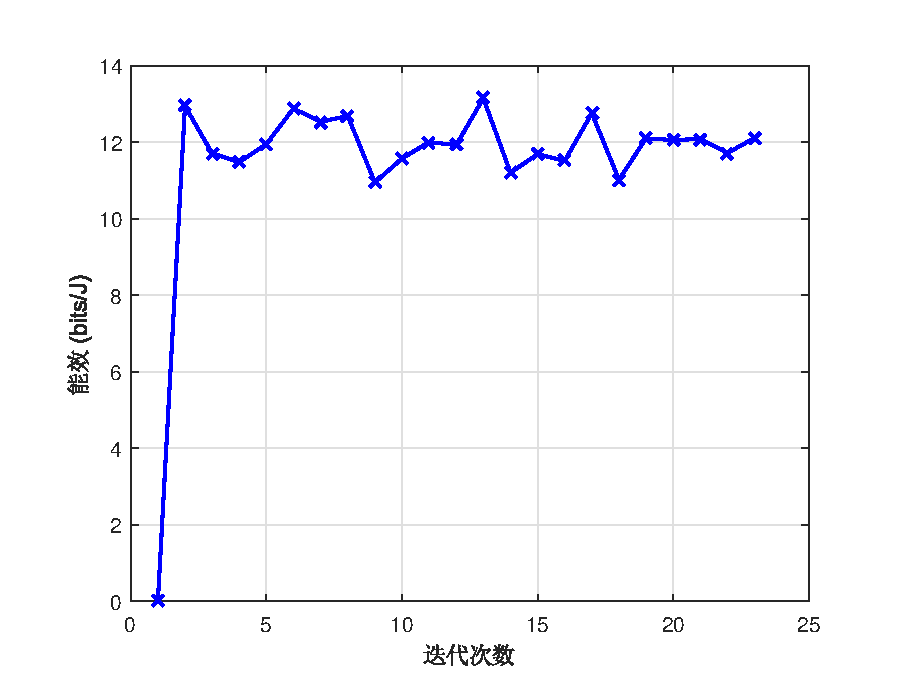
\includegraphics[width=10cm]{figures//chap4//iteration.eps}
\caption{迭代图}
\label{迭代图}
\end{figure}
\end{comment}

首先,展示了不同时隙下的系统总能效最大时的无人机轨迹优化如图 \ref{无人机轨迹优化}所示,其中黑色箭头代表车辆向右行驶为正方向,规定无人机从固定起点飞行至固定终点,
可以发现,当任务时间足够时,无人机会倾向于贴近远离基站的车辆为其服务。图 \ref{无人机速度}展示了无人机在每个时隙的速度情况,当车辆需要无人机辅助时,无人机会放慢速度甚至悬停
以匹配车辆速度为其服务。

\begin{figure}[H]
\centering
\includegraphics[width=16cm,height=8cm]{figures//chap4//小轨迹.eps}   % width=16cm 大字体
\caption{无人机轨迹优化.}
\label{无人机轨迹优化}
\end{figure}

\begin{figure}[H]
\centering
\includegraphics[width=10cm]{figures//chap4//无人机速度.eps}
\caption{无人机速度}
\label{无人机速度}
\end{figure}
在验证了算法的优化轨迹的性能之后,进一步验证了所提方案在不同参数下的性能水平。图 \ref{不同的参数theta下的能效}显示了在使
用不同的 $\theta$ 时,在不同时隙,它们对系统的能效产生了不同的影响。其中$\theta$ 是
描述车辆任务在无人机端与路边单元端的相对能量成本的系数。当 $\theta$ 发生变化时,系统效用也会发生变化。
较高的参数代表了更加关注无人机的飞行能耗。整体的系统能效随着无人机飞行时间 $T$ 的增加而减小,
因为更长的时间足够无人机遍历更多的车辆以获得更好的信道并节省能量。此外,还发现较低的 $\theta$ 会带来较高
的能效。这是因为当认为无人机的的能耗相对重要时,车辆往往会增加功率以传输更多
数据,从而提高能效。
\begin{figure}[H]
\centering
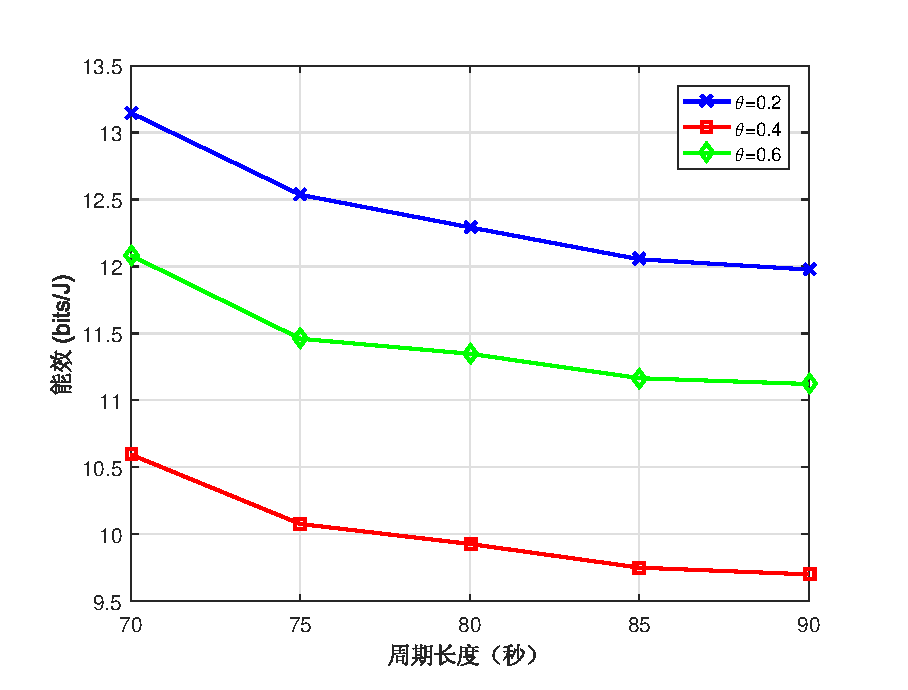
\includegraphics[width=10cm]{figures//chap4//不同的参数theta下的能效.eps}
\caption{不同的参数$\theta$ 下的能效}
\label{不同的参数theta下的能效}
\end{figure}



%\begin{comment}


在图 \ref{不同的方案下的能效}中,对比了固定位置的悬停方案FPHS(Fixed Position Hovering Solution),固定轨迹的方案FTS(Fixed Trajectory Solution)与优化无人机轨迹方案OPTS (Optimized Path Trajectory Solution)
三种无人机通信方案在不同飞行周期$T$下的能效表现。

从整体趋势来看,随着无人机飞行时间的延长,各方案的能效均逐渐趋于稳定,这是因为无人机有了更充足的时间以合适的功率传输数据。
进一步观察发现,OPTS和FPHS两种方案适用于不同的场景。尽管OPTS算法复杂度较高,但它在较短的飞行周期内能够实现更高的能效,显示出更好的时效性。这意味着在需要快速响应的场合,OPTS 是一个优势明显的选择。
相对而言,当飞行周期较长时,FPHS的能效虽然略逊于OPTS,但由于其算法复杂度较低,实现起来更为简单。因此,在时间要求不那么严格的环境中,FPHS 可能是一个更经济的解决方案。
至于FPHS 方案,其能效表现相对较差。这是因为无人机在固定位置悬停,导致与地面车辆之间的距离较远,从而影响了数据传输的效率。此外,随着飞行周期的增加,OPTS和FPHS之间的能效差距逐渐缩小。这主要是因为当飞行周期较短时,OPTS 中的数据传输时间受限,车辆需要在有限的时间内向无人机发送信息,这导致了能效的降低。而随着飞行周期的延长,OPTS 有更多的时间来优化数据传输过程,从而提高了能效。
\begin{comment}
我们分别引入了固定位置的悬停方案FPHS(Fixed Position Hovering Solution),固定轨迹的方案FTS(Fixed Trajectory Solution)与优化无人机轨迹方案OPTS (Optimized Path Trajectory Solution)进行对比
图 \ref{不同的方案下的能效}显示了算法 OPTS、FPHS 和 FTS 在不同无人机飞行周期 $T $下的能效。我们观
察到,由于无人机有足够的时间以适当的功率传输更多的数据,因此在延长无人机飞行周
期时,每个方案的能效都会趋于稳定。注意到 OPTS 和 FHCS 两种算法适用于不同
的情况。具体而言,尽管 OPTS 的复杂度比 FPHS 高,但 OPTS 依然能够在较短周期内
获得更高的能效,这意味着更好的时效性。当周期较长时, FHCS的能效略低于OPTS,
但 FHCS 的复杂度较低,所以在时间敏感度较低的环境中具有优势。
FPHS方案的能效最低,因为无人机悬停在某一固定位置,使无人机和车辆之间的
距离比OPTS和 FTS之间的距离远。很明显,OPTS 和 FHCS  之间的能效差距随着
周期长度增加而缩小,这是由于在OPTS中当飞行
周期较短时,数据传输的剩余时间有限,因此,车辆必须在相对不足的时间内向无
人机发送信息,从而导致较低的能效。
\end{comment}
\begin{figure}[H]
\centering
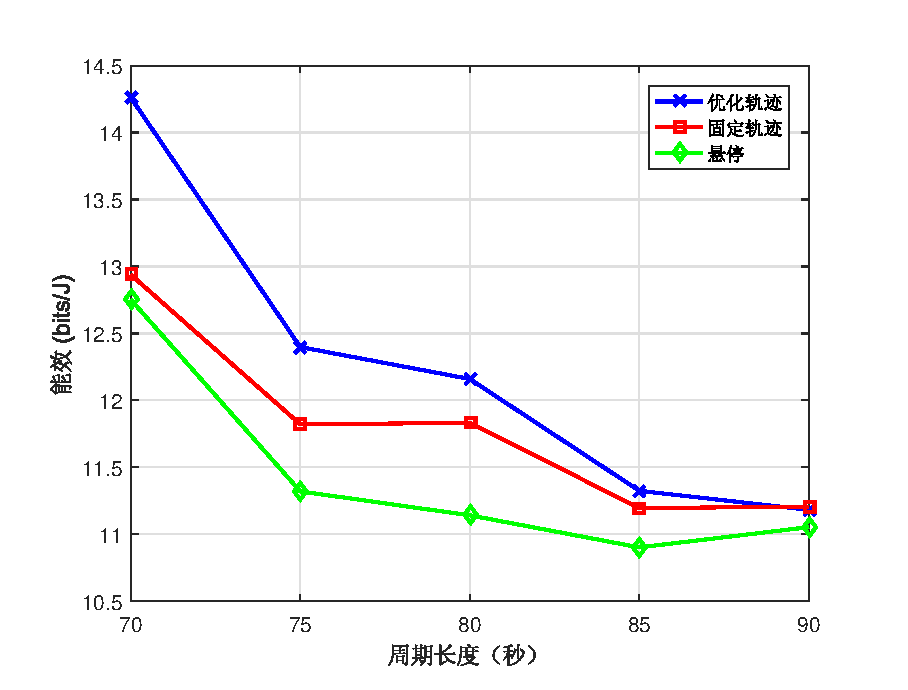
\includegraphics[width=10cm]{figures//chap4//不同的方案下的能效.eps}
\caption{不同的方案下的能效}
\label{不同的方案下的能效}
\end{figure}

下图展示了三种方案在不同参数$\theta$ 下的的对比。在图 \ref{不同的参数在不同的方案下的能效}中,探究了OPTS、FHCS 和FTS三种无人机通信方案的能效如何随参数$\theta$ 的变化而变化。
\begin{figure}[H]
\centering
\includegraphics[width=10cm]{figures//chap4//不同的参数在不同的方案下的能效.eps}
\caption{不同的参数$\theta$ 在不同的方案下的能效}
\label{不同的参数在不同的方案下的能效}
\end{figure}

$\theta$ 是一个关键的参数,它反映了无人机的飞行能耗与通信能耗之间相对能量成本的比重。当$\theta$ 值较大时,无人机的飞行能耗成为整体能耗的主导因素。
观察图中趋势,可以发现,随着$\theta$ 的变化,三种方案的能效都经历了一个明显的下降过程,并在$\theta=0.8$ 时达到最低点。随后,能效呈现出略微上升的趋势。
当$\theta$ 较小时,意味着无人机的飞行能耗在整体能量成本中的占比相对较低。因此,无人机可以更加积极地传输数据,从而提高了整体的能效。相反,当$\theta$ 较大时,无人机的飞行能耗成为主导,这限制了其数据传输的能力,进而影响了能效。
综上所述,参数$\theta$ 通过影响无人机的飞行能耗与通信能耗之间的能量成本分配,进而影响了三种无人机通信方案的能效表现。在实际应用中,需要根据具体场景和需求来选择合适的$\theta$ 值,以优化无人机的通信效率。
\begin{comment}
在图 \ref{不同的参数在不同的方案下的能效}中描述了 OPTS、 FHCS  和 FTS的能效与不同$\theta$ 的关系。注意到$\theta$
是衡量浮标和传感器相对能量成本的一个因素,当θ 值较大时,整个能量消耗由浮标
主导,而传感器则相反。一般来说,三种模式的能效都经历了急剧下降,并在 $\theta=0.8$
时达到最低点;然后呈现略微上升的趋势,原因如下。从浮标的角度来看,较小的θ
意味着浮标的能耗在总成本中相对不太重要;因此,浮标可以传输更多数据以获得
更高的能效。相反,从传感器的角度来看,采用相对较大的θ 有利于传感器发送更多
的数据,同时不会增加太多的总消耗,从而提高能效。

\end{comment}
最后图 \ref{双向车道与单向车道的对比}对比了双向车道场景与单向车道场景,在道路上车辆总数相同的情况下,由于双向车道场景可以更大限度的发挥路边单元与空中基站的协同作用,带来了更高的能效。
\begin{figure}[H]
\centering
\includegraphics[width=10cm]{figures//chap4//双向车道.eps}
\caption{双向车道与单向车道能效对比}
\label{双向车道与单向车道的对比}
\end{figure}
\section{本章小结}\label{section4-6}

在本章中,提出了一种高效的空地一体化的无人机辅助双向车道的车辆通信方案。通过优化车辆的发射功率与无人机的飞行轨迹,以及时隙的分配,
可以使得系统的能效最大化,并通过概率约束,保证了车辆通信的 服务质量,通过调整不同的参数$\theta$,可以发现其可以影响系统的能效。
通过对比不同的无人机飞行方案,能看到优化轨迹的无人机方案最佳。同时,本章也研究了更加现实的方向车道的场景
路边单元与服务器常常部署于道路的一侧,那么在双向车道的场景下,总有一向行驶的车辆势必会远离路边单元,从而造成通信的困难,
使用无人机辅助其通信可以较好的解决该困难。

\begin{comment}
\textcolor[RGB]{18,220,168}{待完善我们联
合优化了发射功率、时隙调度和无人机的轨迹,以最大限度地提高整个网络的能效。
能效最大化问题受到一些传输容量、能量预算和飞行速度的影响;然后采用交替优
化法、丁克尔巴赫方法和基于连续凸逼近的算法进行求解。我们还提出了 FHCS 方
案作为对比对象。虽然 FHCS 的能效总是低于 E2RA 的能效,但 FHCS 由于其较低
的复杂性,更适合于收集周期较长的情形。数值模拟表明,我们的 E2RA 方案在能
效方面的性能明显高于其他对比方案,且可以快速收敛}
\end{comment}


\begin{comment}
表格的引用同样是使用\verb|\ref{}| 命令实现的。例如“表\verb|\ref{tab:ysubof}|” 输出的结果为:表\ref{biao4-1}。\LaTeX 会自动将其替换为表格的编号。例如:
4
的效果如下:\\
注意!从第二章开始应有`` 本章小结",主要总结本章所做的主要研究工作,研究成果等内容!!!


燕山大学硕士学位论文参考文献规则的表格如表\ref{biao4-1} 所示。
%\section{本章小结}\label{section4-7}
\begin{table}[h] %h表示三线表在当前位置插入
\setlength{\abovecaptionskip}{0.05cm} %设置三线表标题与第一条线间距
\centering\small
\caption{{系统仿真参数}}
%\caption{\textbf{The characteristics of various methods}}
%表头文本加黑,但不加黑Table 1. 字样,引入包即可:\usepackage[labelfont=bf]{caption}
%\arrayrulecolor{black} %设置三线表线条颜色:黑色
\begin{tabular*}{\hsize}{@{\extracolsep{\fill}}c c c c} %{\hsize} 使三线表自适应宽度,c表示文本居中
  \hline
  参数 & 数值 \\
  \hline
  人机高度  & 100 \\
  1地面基站高度 & 222  \\
  地面基站高度面基站高度面基站高度面基站高度  & 2222  \\
  \hline
\end{tabular*}
\end{table}
\end{comment}

\begin{comment}
\begin{table}[h] %h表示三线表在当前位置插入
\setlength{\abovecaptionskip}{0.05cm} %设置三线表标题与第一条线间距
\centering\small
\caption{{系统仿真参数}}
%\caption{\textbf{The characteristics of various methods}}
%表头文本加黑,但不加黑Table 1. 字样,引入包即可:\usepackage[labelfont=bf]{caption}
%\arrayrulecolor{black} %设置三线表线条颜色:黑色
\begin{tabular*}{\hsize}{@{\extracolsep{\fill}}c c c c} %{\hsize} 使三线表自适应宽度,c表示文本居中
  \hline
  参数 & 数值 \\
  \hline
  人机高度  & 100 \\
  1地面基站高度 & 222  \\
  地面基站高度面基站高度面基站高度面基站高度  & 2222  \\
  \hline
\end{tabular*}
\end{table}
\end{comment}

\begin{comment}
\begin{equation}
\begin{aligned}
\max _{ \boldsymbol{P}, \boldsymbol{Q}} & EE(\boldsymbol{P},\boldsymbol{Q}) \\
\text { s.t. }
& Pr\left\{x_m\left[t\right]SNR_{m,R}\left[t\right]+y_m\left[t\right]SNR_{m,U}\left[t\right]\geq S N R_{th}\right\}\geq1-\varepsilon_1, \forall m,t \\
& q_U^{n\mathrm{\ }+1}-q_U^{n\mathrm{\ }}\le tV_{max}, \forall m \\
& x_m\left[t\right] + y_m\left[t\right]=1, \forall m\\
& 0\le p_m\left[t\right]\le p_{max}, \forall m
\end{aligned}
\end{equation}

\begin{eqnarray}
\begin{aligned}
\max _{ \boldsymbol{P}, \boldsymbol{Q}} & EE(\boldsymbol{P},\boldsymbol{Q}) \label{equ-s1a}\\
\text { s.t. }
& Pr\left\{x_m\left[t\right]SNR_{m,R}\left[t\right]+y_m\left[t\right]SNR_{m,U}\left[t\right]\geq S N R_{th}\right\}\geq1-\varepsilon_1, \forall m,t  \label{equ-s2a}\\
& q_U^{n\mathrm{\ }+1}-q_U^{n\mathrm{\ }}\le tV_{max}, \forall m  \label{equ-s3a}\\
& x_m\left[t\right] + y_m\left[t\right]=1, \forall m \label{equ-s4a}\\
& 0\le p_m\left[t\right]\le p_{max}, \forall m  \label{equ-v1a}
\end{aligned}
\end{eqnarray}

\begin{align}
\max _{ \boldsymbol{P}, \boldsymbol{Q}} & EE(\boldsymbol{P},\boldsymbol{Q}) \label{equ-s1a}\\
\text { s.t. }
& Pr\left\{x_m\left[t\right]SNR_{m,R}\left[t\right]+y_m\left[t\right]SNR_{m,U}\left[t\right]\geq S N R_{th}\right\}\geq1-\varepsilon_1, \forall m,t  \label{equ-s2a}\\
& q_U^{n\mathrm{\ }+1}-q_U^{n\mathrm{\ }}\le tV_{max}, \forall m  \label{equ-s3a}\\
& x_m\left[t\right] + y_m\left[t\right]=1, \forall m \label{equ-s4a}\\
& 0\le p_m\left[t\right]\le p_{max}, \forall m  \label{equ-v1a}
\end{align}

\begin{align}
\max _{ \boldsymbol{P}, \boldsymbol{Q}} & EE(\boldsymbol{P},\boldsymbol{Q}) \label{YY}\\
\text { s.t. }
& Pr\left\{x_m\left[t\right]SNR_{m,R}\left[t\right]+y_m\left[t\right]SNR_{m,U}\left[t\right]\geq S N R_{th}\right\}\geq1-\varepsilon_1, \forall m,t  \label{YYa}\\
& q_U^{n\mathrm{\ }+1}-q_U^{n\mathrm{\ }}\le tV_{max}, \forall m  \label{YYb}\\
& x_m\left[t\right] + y_m\left[t\right]=1, \forall m \label{YYc}\\
& 0\le p_m\left[t\right]\le p_{max}, \forall m  \label{equ-v1a}
\end{align}

\begin{subequations}
\renewcommand{\theequation}
{\theparentequation-\arabic{equation}}
\begin{equation}
A = B
\end{equation}
\begin{equation}
C = D
\end{equation}
\end{subequations}

\end{comment}
